\documentclass{article}
\usepackage{tikz}

\begin{document}
	\begin{center}
		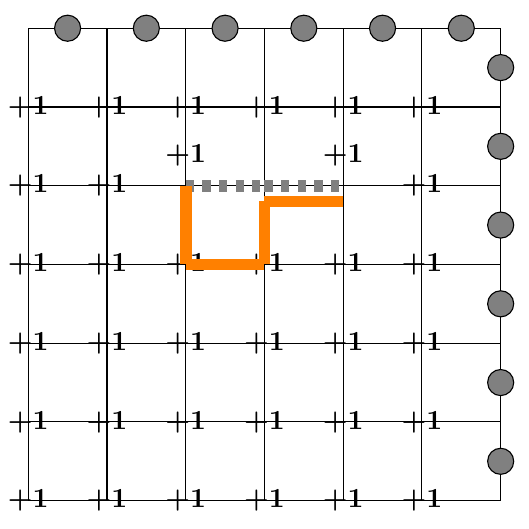
\begin{tikzpicture}
			
			
			
			% Draw solid grid and nodes with circles in the middle of each side
			\draw[step=1cm] (-3,-3) grid (3,3);
			\foreach \i in {-2.5,...,2.5}
			{
				\foreach \j in {-2.5,...,2.5}
				{
					
					
					\begin{scope}[transform canvas={xshift=\i cm,yshift=\j cm}]
						
						\node[right,xshift=0.2cm,yshift=0.4cm] {};
						% Convert \j and \i to integers
						\pgfmathtruncatemacro{\intj}{\j}
						\pgfmathtruncatemacro{\inti}{\i}
						
						\ifnum\intj=2
						\draw node[draw,circle,fill=gray] at (0,0.5) {};
						\fi
						
						\ifnum\inti=2
						\draw node[draw,circle,fill=gray] at (0.5,0) {};
						\fi
						
						
						
						\ifnum\intj=1
						\ifnum \inti=0
						\draw node[label=center:\textbf{}] at (-0.5,0) {};
						\draw node[label=center:\textbf{}] at (0.5,0) {};
						\else
						\ifnum \inti>1
						\draw node[label=center:\textbf{+1}] at (-0.5,-0.5) {};
						\fi
						\ifnum \inti<1
						\draw node[label=center:\textbf{+1}] at (-0.5,-0.5) {};
						\fi
						\fi
						\else
						\draw node[label=center:\textbf{+1}] at (-0.5,-0.5) {};
						\fi
						
					\end{scope}
				}
			}
			
			
			\foreach \j in {1,...,1}
			{
				%\draw[black!50, line width=1.5mm] (-2, \j) -- (-1.5, \j);
				\draw[dashed,black!50, line width=1.5mm] (-1, \j) -- (0, \j);
				\draw node[label=north:\textbf{+1}] at (-1,\j) {};
				\draw[dashed, black!50, line width=1.5mm] (0, \j) -- (1, \j);
				\draw node[label=north:\textbf{+1}] at (1,\j) {};
				
			}
			
			\foreach \j in {0.8,...,0.8}
			{
	
				\draw[orange, line width=1.5mm] (0, \j) -- (1, \j);
				
			}
			
			\foreach \i in {-1,...,-1}
			{
				
				\draw[orange, line width=1.5mm] (\i,0) -- (\i, 1 );
				
			}
			
				\foreach \i in {0,...,0}
			{
				
				\draw[orange, line width=1.5mm] (\i,0) -- (\i, 0.8 );
				
			}
			
				\foreach \j in {0,...,0}
			{
				
				\draw[orange, line width=1.5mm] (-1,\j) -- (0,\j);
				
			}
			
			
			
		\end{tikzpicture}
	\end{center}
	
\end{document}
